
\documentclass[12pt]{article}
%% preamble.tex

% enclose any latex in \comment{} to suppress it
\newcommand{\comment}[1]{}
\newcommand{\citeNP}[1]{\cite{#1}}

\usepackage{graphicx}
\usepackage{multicol}
\usepackage{times}
\usepackage{floatflt}
\graphicspath{{./}{figures/}}

% NO psfig -- pdflatex does not support it ...
% \usepackage{psfig}
% \psfigurepath{./:figures/}
% \DeclareGraphicsRule{.eps.gz}{eps}{.eps.bb}{'gunzip -c #1}

\newcommand{\upline}{\vspace*{-\baselineskip}}
\newcommand{\up}{\vspace*{-6pt}}
\newcommand{\downline}{\vspace*{\baselineskip}}
\newcommand{\sep}{~~~~~~~~~~}

% this hardcodes the bib name, which we don't want to do.
% \renewcommand{\thebibliography}[1]{\section*{References Cited}
% \addcontentsline{toc}{section}{References Cited}\list
%  {[\arabic{enumi}]}{\settowidth\labelwidth{[#1]}\leftmargin\labelwidth
%  \advance\leftmargin\labelsep
%  \usecounter{enumi}}
%  \def\newblock{\hskip .11em plus .33em minus -.07em}
%  \sloppy\clubpenalty4000\widowpenalty4000
%  \sfcode`\.=1000\relax}

% fix this to specify width and height, and solve for the margins
% margins.tex

% import calc
\usepackage{calc}

%
\newlength{\myrightmargin}
\newlength{\myleftmargin}
\newlength{\mytopmargin}
\newlength{\mybottommargin}

% Change these settings to change the margins
\setlength{\myrightmargin}{1.0in}
\setlength{\myleftmargin}{1.0in}
\setlength{\mytopmargin}{0.75in}     
\setlength{\mybottommargin}{0.75in} 
\setlength{\oddsidemargin}{0.0in}   % extra room on inside side

%%% use margin settings to set width variables
\setlength{\evensidemargin}{0 in}
\setlength{\marginparsep}{0 in}
\setlength{\marginparwidth}{0 in}
\setlength{\hoffset}{\myleftmargin - 1.0in}
\setlength{\textwidth}
  {8.5in -\myleftmargin -\myrightmargin -\oddsidemargin}

%%% use margin settings to set height variables
\setlength{\voffset}{\mytopmargin -1.0in}
\setlength{\topmargin}{0 in}
\setlength{\headheight}{12 pt}
\setlength{\headsep}{20 pt}
\setlength{\footskip}{36 pt}
\setlength{\textheight}
  {11.0in-\mytopmargin-\mybottommargin-\headheight-\headsep-\footskip}

% \oddsidemargin 0.2cm
% \evensidemargin 0cm
% \textwidth 16.0cm
% \topmargin -1.25cm
% \textheight 22.94cm

% remove parindent, squeeze grafs
\setlength{\parindent}{0in}
\setlength{\parskip}{1ex}

\def\nibf#1{\noindent\textbf{#1}}

\usepackage{multirow}
\usepackage{amsmath}
\usepackage{fancyhdr}
\usepackage[left=1in,top=1.0in,right=1in,headsep=0.25in,footskip=0.3in,bottom=0.7in]{geometry}
%\usepackage[left=1in,top=1.2in,right=1in,footskip=0.3in,bottom=0.7in,showframe]{geometry}
%\usepackage[left=1in,top=1in,right=1in,bottom=1in,nohead]{geometry}
\usepackage{graphicx}
\renewcommand{\arraystretch}{1} % spacing between table rows
\usepackage[]{caption}
\setlength{\abovecaptionskip}{0pt}
\setlength{\belowcaptionskip}{-5pt}
\setlength{\intextsep}{10pt plus 2pt minus 2pt}
\usepackage[normalem]{ulem}
\newcounter{Labcounter}
\newcounter{Taskcounter}
\numberwithin{equation}{section}
\fancyhf{}
\pagestyle{fancy}
\fancypagestyle{plain}{ %
% \fancyhf{} % remove everything
\renewcommand{\headrulewidth}{0pt} % remove lines as well
%\renewcommand{\footrulewidth}{0pt}
%\cfoot{Page \thepage~of \pageref{LastPage}}}
\cfoot{\thepage}
}


\lhead{\textit{Nanospheres...}}
%\chead{\Large \textbf{Paul W.~Leu } \vspace{0.3em}}
%\chead{\Large \textbf{NSF Biographical Sketch: Paul W.~Leu} \vspace{0.3em}}
\rhead{\textit{Leu}}
\newcommand{\blue}[1]{\textcolor{blue}{#1}} %for displaying red texts

\newcommand{\vectornorm}[1]{\left|\left|#1\right|\right|}
%\usepackage[top=2.5cm, bottom=2.5cm, left=2.5cm, right=2.5cm]{geometry}
\usepackage[normalem]{ulem}
\newenvironment{packed_enum}{
\begin{enumerate}
  \setlength{\topsep}{0pt}
  \setlength{\partopsep}{0pt}
  \setlength{\itemsep}{1pt}
  \setlength{\parskip}{0pt}
  \setlength{\parsep}{0pt}
}{\end{enumerate}}

%\usepackage[small]{caption}
\usepackage[draft]{pdfcomment}
\usepackage{wrapfig}
\usepackage{hyperref}
\usepackage{paralist}
\usepackage{amsmath}
\usepackage{amssymb}
\usepackage{amsfonts}
\usepackage{textcomp}
\usepackage{subfig}
\usepackage{framed}
\usepackage{setspace}
\usepackage{here}
\usepackage[numbers, square, comma, sort&compress]{natbib}

\usepackage[compact]{titlesec}
\titlespacing{\section}{0pt}{0ex}{0pt}
\titlespacing{\subsection}{0pt}{0pt}{0pt}
\usepackage{xcolor}

\usepackage[]{caption}
\setlength{\abovecaptionskip}{0pt}
\setlength{\belowcaptionskip}{-5pt}
\setlength{\intextsep}{10pt plus 2pt minus 2pt}


\usepackage{float}
\floatstyle{plaintop}
\newfloat{program}{thp}{lop}
\floatname{program}{Table}

\newfloat{wrapprogram}{thp}{lop}
\floatname{wrapprogram}{Table}

%\setlength{\intextsep}{10pt plus 2pt minus 2pt}
% bold face: highlight keywords, or big ideas
% italics: inconspicuous stressing of key points
% underline: hypothesis; avoid

\usepackage{bm}

\date{\today }

\author{
Paul W. Leu\\
University of Pittsburgh\\
Pittsburgh, PA}


%\def\myTitle{CAREER: Transforming Solar Energy Harvesting through Nanophotonic Light Trapping}
%\def\myTitle{CAREER: Characterizing Enhanced Absorption and Carrier Collection Mechanisms in Silicon and Zinc Oxide Nanocone-based Solar Cells}
%Upper bound
%   100 hours/year
%    40 hours
%    
%\title{Ultimate Limits of Silicon Nanostructures for Photon Management\\
%\title{Determining Silicon/Metal Nanostructures that Approach the Wave-Optics Light Trapping Limit by Data Mining of Electrodynamic Simulations}
%\title{CAREER: Characterizing Enhanced Absorption and Carrier Collection Mechanisms in Silicon and Zinc Oxide Nanocone-based Solar Cells}
%\title{Predicting Wave-Optics Light Trapping in Silicon and Metal Nanostructure by Data Mining of Electrodynamic Simulations}
%Keywords: ultra thin, light trapping, wave-optics light trapping, coherent light trapping, optimization framework, data mining}

%\title{Modeling and Manufacturing of Three Dimensional Silicon Nanostructures for Photon Management}

\begin{document}

\tableofcontents

\section{Leaky Waveguide Modes}

\subsection{TE}
\blue{Why use this convention as opposed to in Yariv and Yeh?  In Yariv and Yeh, 
outside the semiconductor, 
$k_{1x} = \left [  \beta^2  -  \left ( \frac{n_1 \omega}{c} \right )^2  \right ] ^{1/2}$.  Since $\beta >  \frac{n_1 \omega}{c}$, $k_{1x}$ is real.
In this derivation, $k_{1x}$ must be imaginary to be confined.  Yariv and Yeh focuses on guided modes, where as this is for leaky waveguide modes.}\\
$k_{1x} = \left [  \left ( \frac{n_1 \omega}{c} \right )^2 - \beta^2    \right ] ^{1/2}$
and 
$k_{2x} = \left [  \left ( \frac{n_2 \omega}{c} \right )^2 - \beta^2    \right ] ^{1/2}$.  

For TE modes, there are only components $E_y$, $H_x$, $H_z$.  $E_y$ is out of plane.  
For even mode, $\mathbf{H}(- \mathbf{r}) = \mathbf{H} ( \mathbf{r} )$ and 
$- \mathbf{E}(- \mathbf{r}) = \mathbf{E} ( \mathbf{r} )$.
\begin{equation}
\hat{O}_{M_x} \mathbf{E} (\mathbf{r}) = M_x \mathbf{E} ( M_x \mathbf{r})
\end{equation}
$(E_x, E_y, E_z) (x, y, z) = (-E_x, E_y, E_z) (-x, y, z) $.

For even TE modes, $E_y$ is the same above and below the midplane of the thin film or $x = 0$.  
$E_y (x, y, z) = E_y (-x, y, z) $.  Thus, for even TE modes
\begin{equation}
i k_{2x} \tan (k_{2x} \frac{1}{2} d ) = k_x
\end{equation}
and 
\begin{equation}
k_x^2 + k_{2x}^2 = V
\end{equation}


or 
\begin{equation}
\boxed{\tan (k_{2x} \frac{1}{2} d ) = - i \frac{k_x}{k_{2x}}.}
\end{equation}


For odd modes, 
$-\mathbf{H}(- \mathbf{r}) = \mathbf{H} ( \mathbf{r} )$ and 
$\mathbf{E}(- \mathbf{r}) = \mathbf{E} (\mathbf{r} )$.  
\begin{equation}
\hat{O}_{M_x} \mathbf{E} (\mathbf{r}) = - M_x \mathbf{E} ( M_x \mathbf{r})
\end{equation}
$(E_x, E_y, E_z) (x, y, z) = (E_x, -E_y, -E_z) (-x, y, z) $.

For TE modes, $E_y$ has a sign change about the midplane of the thin film or $x = 0$. 
$E_y (x, y, z) = -E_y (-x, y, z) $.
For odd TE modes,
\begin{equation}
\boxed{k_{2x} \cot (k_{2x} \frac{1}{2} d ) = i k_x}
\end{equation}

The two equations can be combined 
\begin{equation}
\tan (k_{2x} d )  = - \frac{ i 2 k_x k_{2x}}{( k_{2x}^2 + k_x^2 )} 
\end{equation}

\subsection{TM}
For TM modes, there are only components $H_y$, $E_x$, $E_z$.  $H_y$ is out of plane.  
For even modes, $\mathbf{H}(- \mathbf{r}) = \mathbf{H} ( \mathbf{r} )$
\begin{equation}
\hat{O}_{M_x} \mathbf{H} (\mathbf{r}) = M_x \mathbf{H} ( M_x \mathbf{r})
\end{equation}
$(H_x, H_y, H_z) (x, y, z) = -(-H_x, H_y, H_z) (-x, y, z) = (H_x, -H_y, -H_z) (-x, y, z)$
For TM modes, $H_y$ is the flipped above and below the midplane of the thin film or $x = 0$.  
$H_y (x, y, z) = -H_y (-x, y, z) $.

For TM modes, $E_y$ has a sign change about the midplane of the thin film or $x = 0$. 
The solution is 
\begin{equation}
\boxed{k_{2x} \cot (k_{2x} \frac{1}{2} d ) = i \frac{n_2^2}{n_1^2} k_x }
\end{equation}


For odd modes, $\mathbf{H}(- \mathbf{r}) = - \mathbf{H} ( \mathbf{r} )$
\begin{equation}
\hat{O}_{M_x} \mathbf{H} (\mathbf{r}) = - M_x \mathbf{H} ( M_x \mathbf{r})
\end{equation}
$(H_x, H_y, H_z) (x, y, z) = -(-H_x, H_y, H_z) (-x, y, z) = (H_x, -H_y, -H_z) (-x, y, z)$.
For TM modes, $H_y$ is the same above and below the midplane of the thin film or $x = 0$.  
$H_y (x, y, z) = H_y (-x, y, z) $.
\begin{equation}
\boxed{i k_{2x}\tan (k_{2x} \frac{1}{2} d ) = \frac{{n_2^2}}{n_1^2} k_x}
\end{equation}


\blue{The way it is described in some textbooks, TM even means $H_y$ is even and TM odd means $H_y$ is odd.  However, since $H$ is a pseudovector, 
these definitions should be flipped.}  


The two equations can be combined to be
\begin{equation}
\tan (k_{2x} d )  = - \frac{ i 2 \bar{k_x} k_{2x}}{( k_{2x}^2 + \bar{k_x}^2 )} \\
\end{equation}
where 
\begin{equation}
\bar{k_x} = \frac{{n_2^2}}{n_1^2} k_x
\end{equation}

\subsection{Normal Incidence; $\beta = 0$}

At normal incidence, 
the even TE mode becomes
\begin{equation}
\begin{aligned}
n_2 k \tan (n_2 k \frac{1}{2} d ) & = - i n_1 k \\ 
\tan (n_2 k \frac{1}{2} d ) & = - i  \frac{n_1}{n_2}
\end{aligned}
\end{equation}
where $k = \frac{\omega}{c}$.
\begin{equation}
\boxed{\cot (n_2 k \frac{1}{2} d ) = i \frac{n_2}{n_1} }
\end{equation}
The odd TE mode becomes
\begin{equation}
\boxed{\tan (n_2 k \frac{1}{2} d ) = - i \frac{n_2}{n_1} }
\end{equation}

The TM modes result in the same equations for $\beta = 0$.  
These equations are the same as in Linyou's, except for the 1/2 \cite{Yu:12}.  



%\uline{These expressions match Linyou's, except for the 1/2.}
%
%\subsection{Waveguide Modes}
%For TE modes, 
%\begin{equation}
%%\begin{aligned}
%\tan (k_{2x} d )  = - \frac{ i 2 k_x k_{2x}}{( k_{2x}^2 + k_x^2 )} \\
%%\end{aligned}
%\end{equation}
%
%For TM modes, 
%\begin{equation}
%\tan (k_{2x} d )  = - \frac{ i 2 \bar{k_x} k_{2x}}{( k_{2x}^2 + \bar{k_x}^2 )} \\
%\end{equation}
%where 
%\begin{equation}
%\bar{k_x} = \frac{{n_2^2}}{n_1^2} k_x
%\end{equation}

\subsection{Pala}

Following \cite{Pala:09}, the solution to 50 nm Si waveguide modes with SiO$_2$ on both sides is.
Use script \texttt{Pala.m}. 

\begin{figure}[H]
\centering 
\vspace{-10pt}
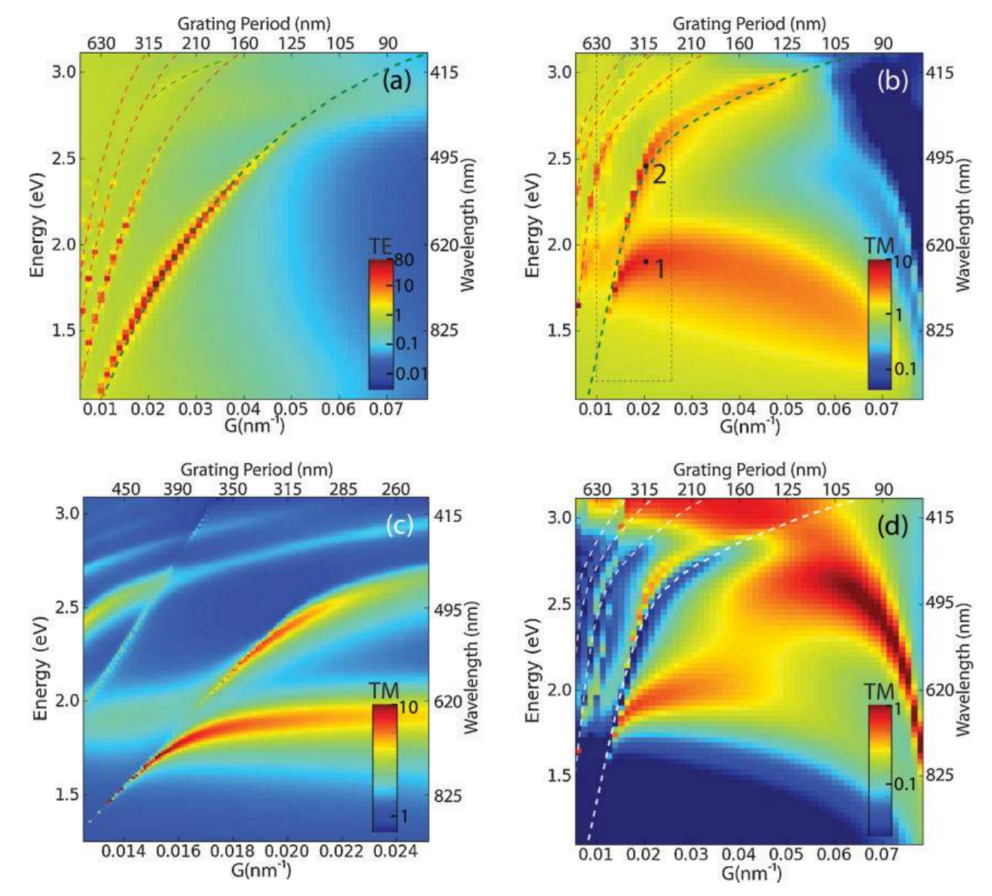
\includegraphics[scale=.5]{Figures/PalaFigure}
\caption{(a) TE illumination.  (b) TM illumination.}
%\vspace{-10pt}
\end{figure}

\begin{figure}[H]
\centering 
\vspace{-10pt}
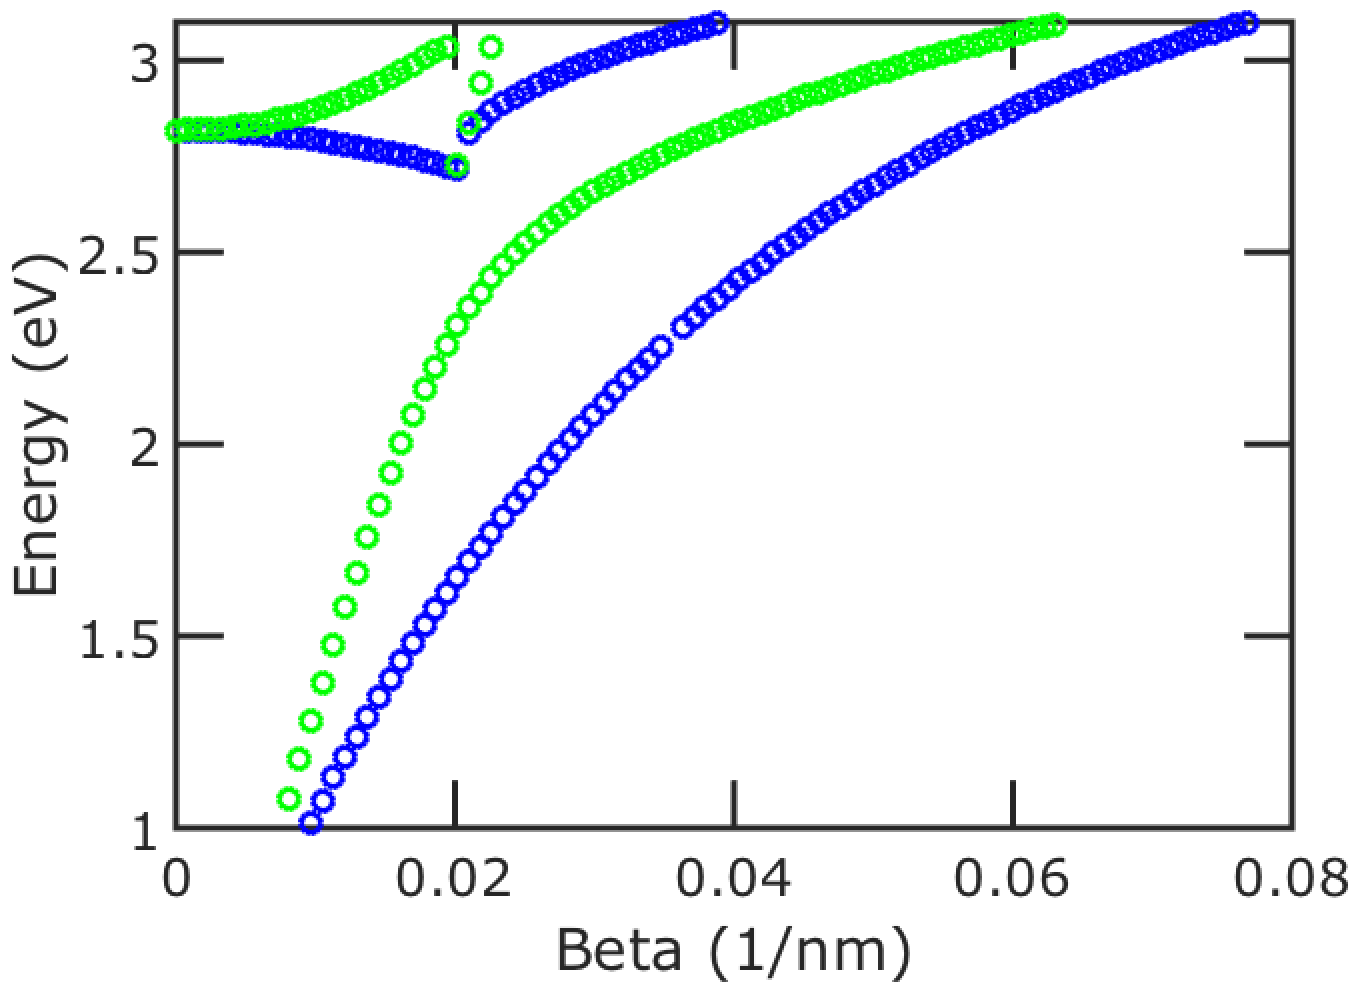
\includegraphics[scale=.27]{Figures/PalaModes}
\caption{Leaky TE Modes in blue, TM modes in green}
%\vspace{-10pt}
\end{figure}

\begin{figure}[H]
\centering 
\vspace{-10pt}
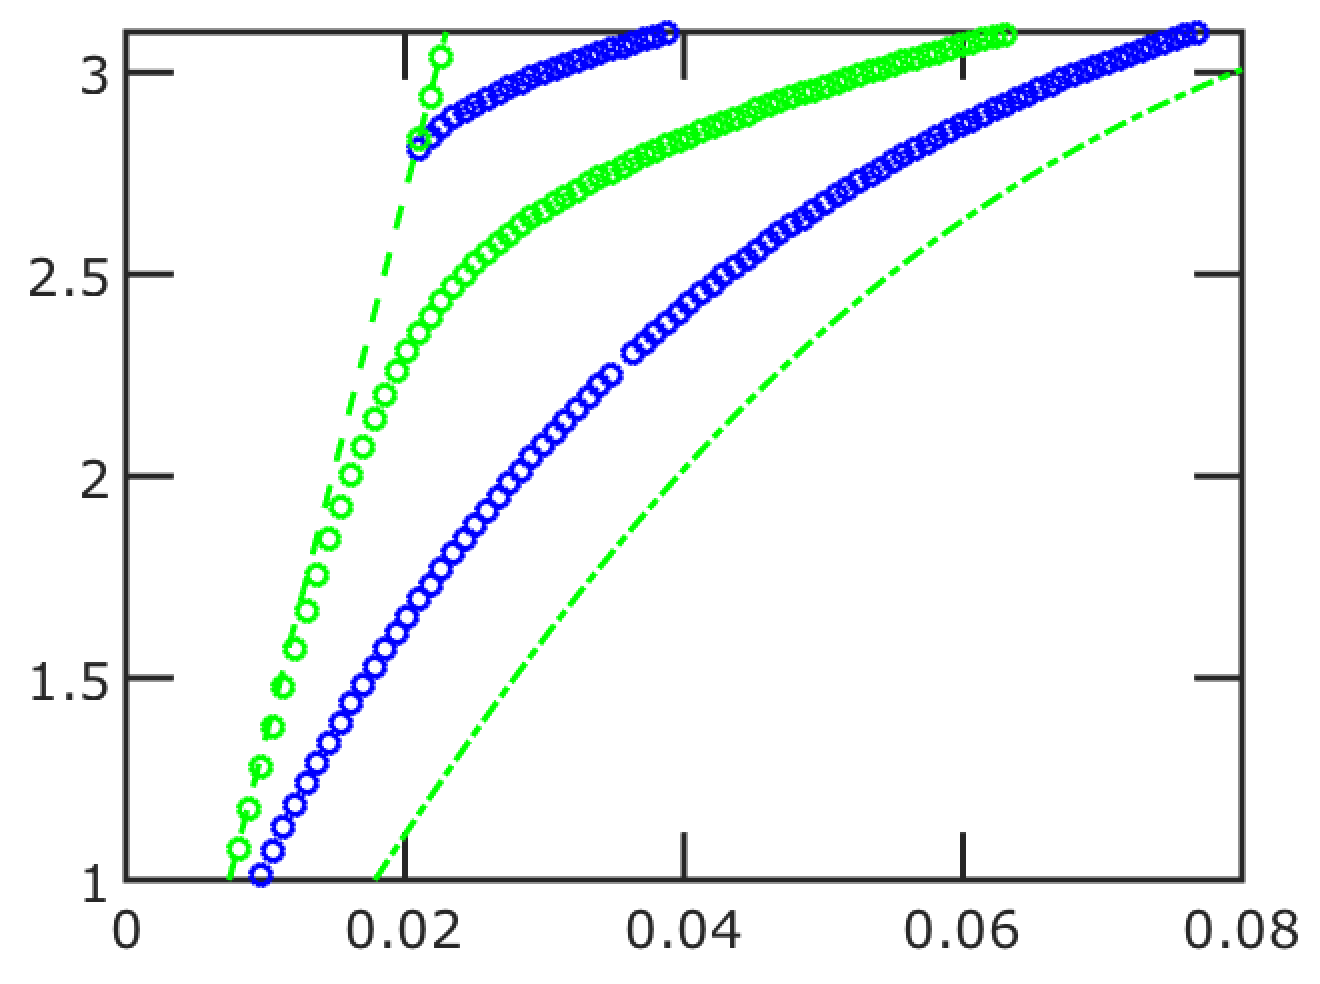
\includegraphics[scale=.27]{Figures/PalaModesWaveguide}
\caption{Guided TE Modes in blue, TM modes in green using Yariv's equations}
\vspace{-10pt}
\end{figure}


\subsection{Joannopoulos}

\begin{figure}[H]
\centering 
\vspace{-10pt}
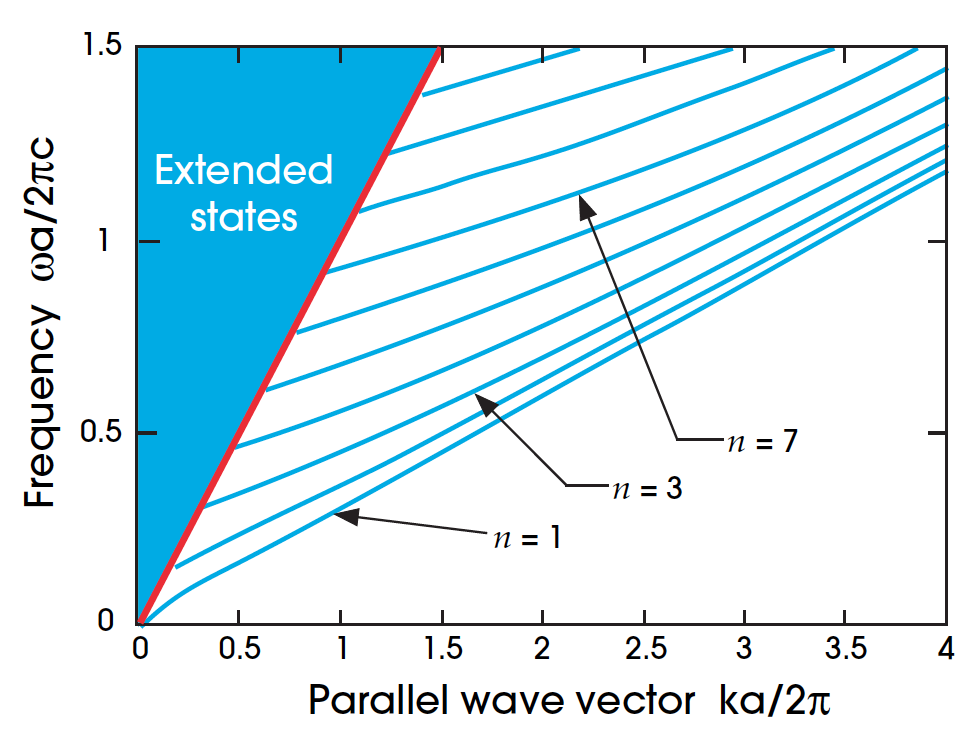
\includegraphics[scale=.4]{Figures/Joannopoulos}
\caption{Figure from paper.}
\vspace{-10pt}
\end{figure}

We try to duplicate this with $a = 50$ nm.  I
The minimum $\omega = 0$.  
The maximum $\omega = $

\begin{figure}[H]
\centering 
\vspace{-10pt}
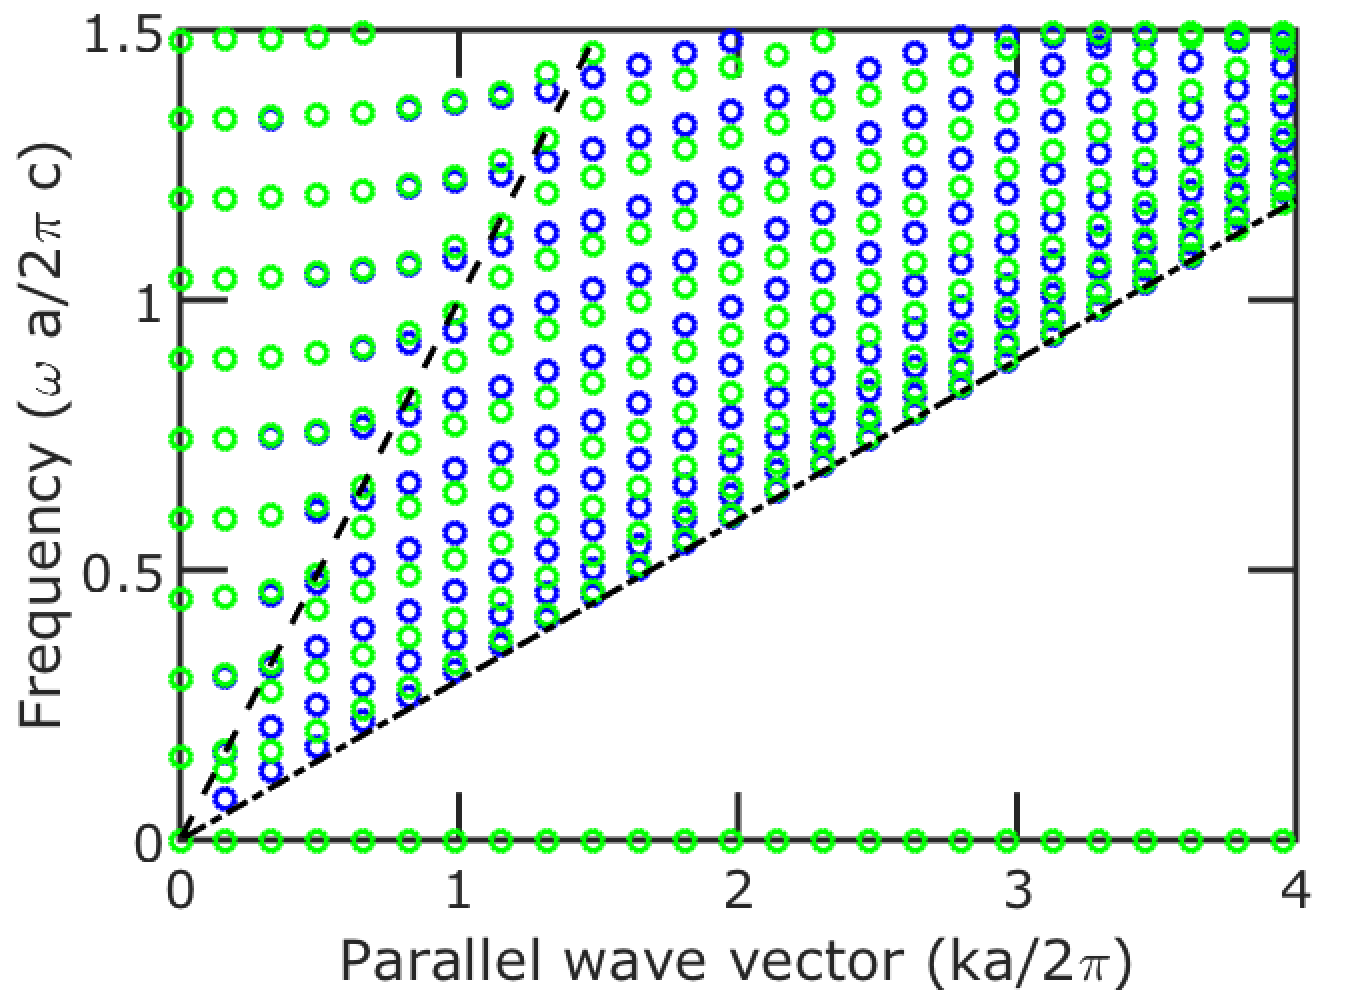
\includegraphics[scale=.4]{Figures/JoannopoulosFigure}
\caption{Figure from paper.}
\vspace{-10pt}
\end{figure}

\section{With back metal}

For TE modes, 
\begin{equation}
\boxed{k_{2x} \cot (k_{2x} d ) = i k_x}
\end{equation}
The equation is just like the equation for an odd TE mode except that 
the thickness is now $d$ instead of $d/2$ in the equation.  
This intuitively makes sense since the $E_y = 0$ at $x = 0$.  Thus, only the odd TE solutions from before are possible.  

For TM modes, 
\begin{equation}
\boxed{i k_{2x}\tan (k_{2x} d ) = \frac{{n_2^2}}{n_1^2} k_x}
\end{equation}
The equation is just like the equation for an odd TE mode except that 
the thickness is now $d$ instead of $d/2$ in the equation.  
This intuitively makes sense since the $E_y = 0$ at $x = 0$.  Thus, only the odd TE solutions from before are possible.  
\subsection{Normal Incidence}

In the limit $\beta \rightarrow 0$, $k_x = n_1 k$ and $k_{2x} = n_2 k$.
\begin{equation}
\boxed{\tan (n_2 k d) = - i \frac{n_2}{n_1} }
\end{equation}
This is just the odd mode before with thickness $d$ instead of $d/2$.  

\subsection{Our Hemisphere Paper}

This calculates the waveguide modes for 100 nm thick Si on metal.
Use script \texttt{Gao\_Hemisphere.m}.

\begin{figure}[H]
\centering 
\vspace{-10pt}
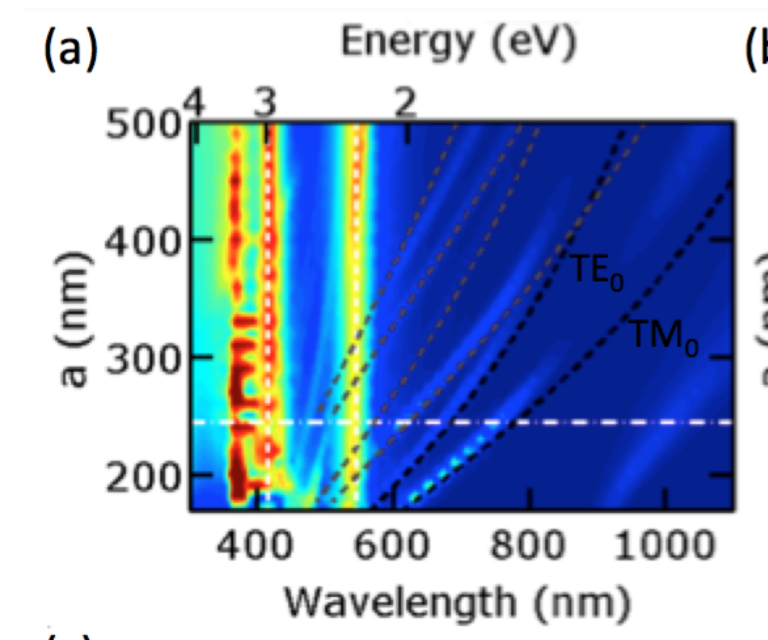
\includegraphics[scale=.4]{Figures/HemispherePaperFigure}
\caption{Figure from paper.}
\vspace{-10pt}
\end{figure}

\begin{figure}[H]
\centering 
%\vspace{-10pt}
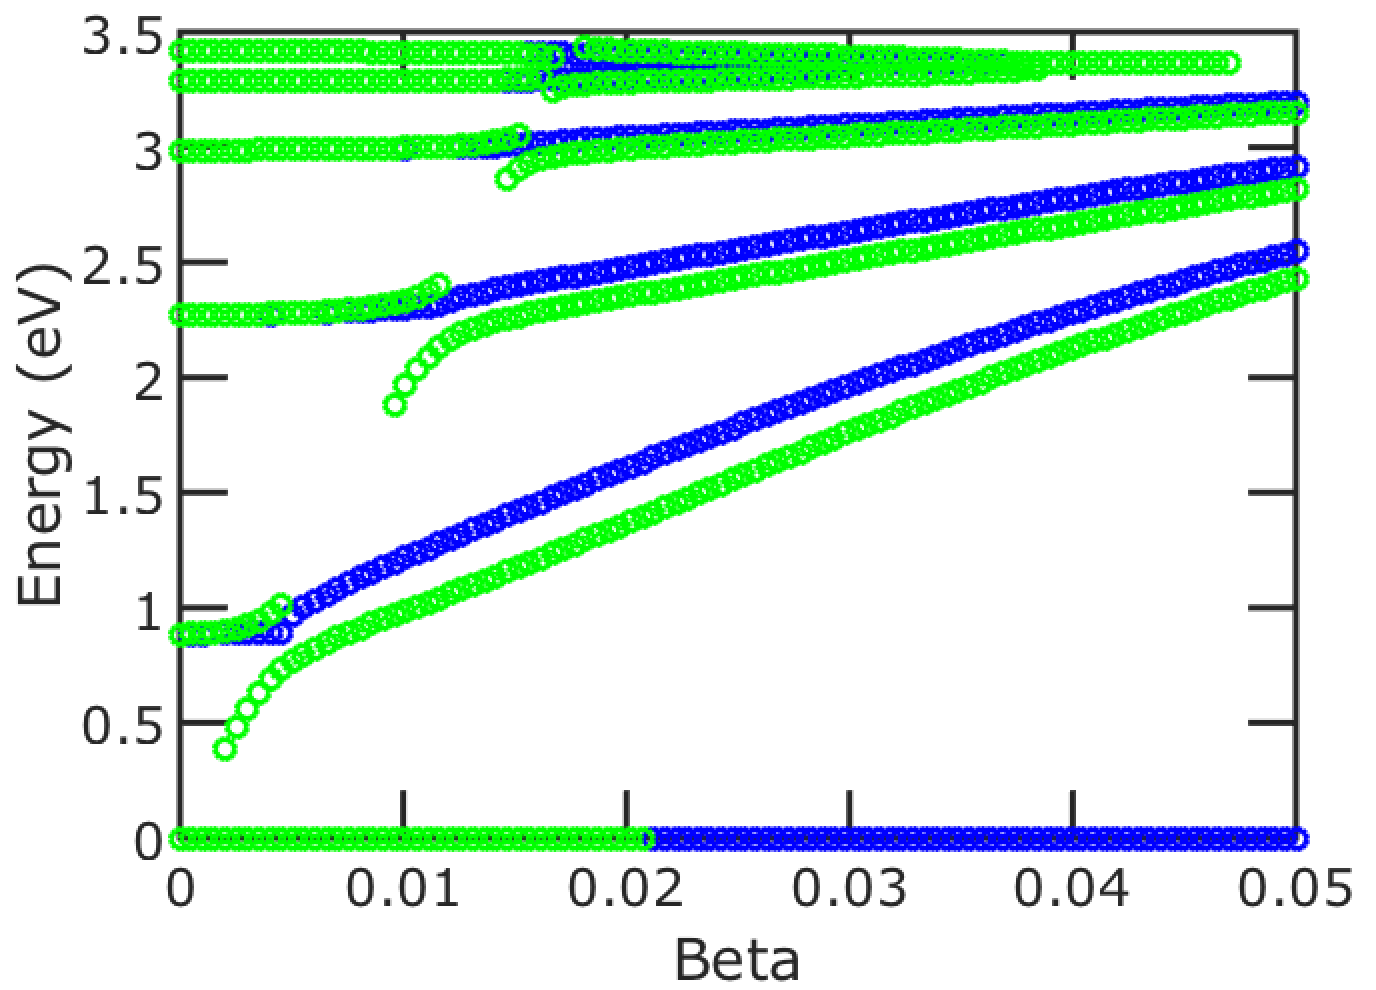
\includegraphics[scale=.4]{Figures/HemispherePaper}
\caption{Leaky TE Modes in blue.  TM modes in green.}
%\vspace{-10pt}
\end{figure}

\begin{figure}[H]
\centering 
%\vspace{-10pt}
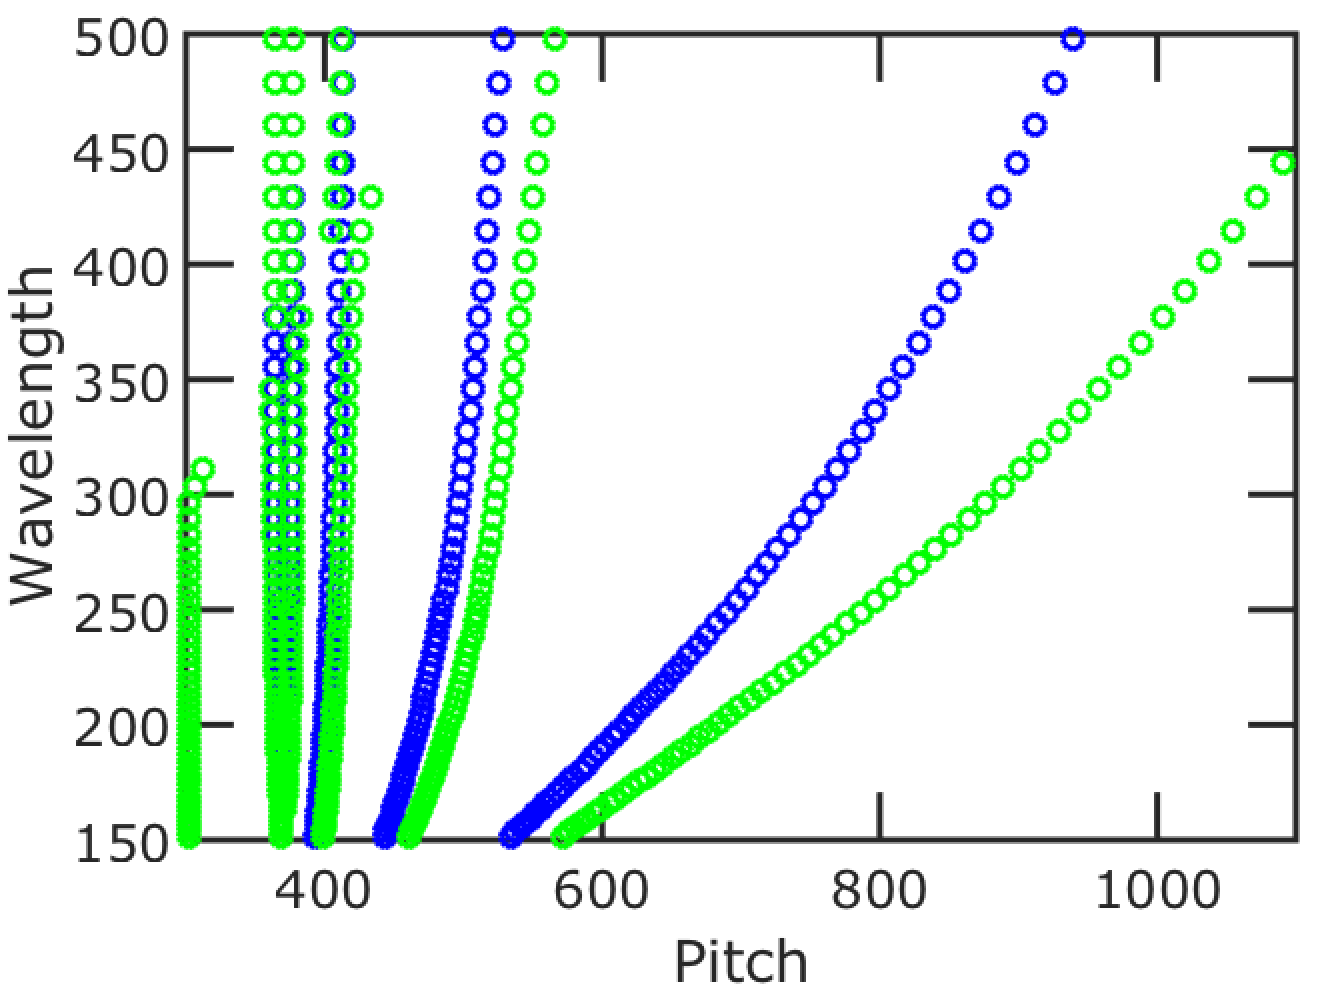
\includegraphics[scale=.4]{Figures/HemispherePaperWavelength}
\caption{Leaky TE modes in blue.  Leaky TM modes in green.}
%\vspace{-10pt}
\end{figure}

\begin{figure}[H]
\centering 
\vspace{-10pt}
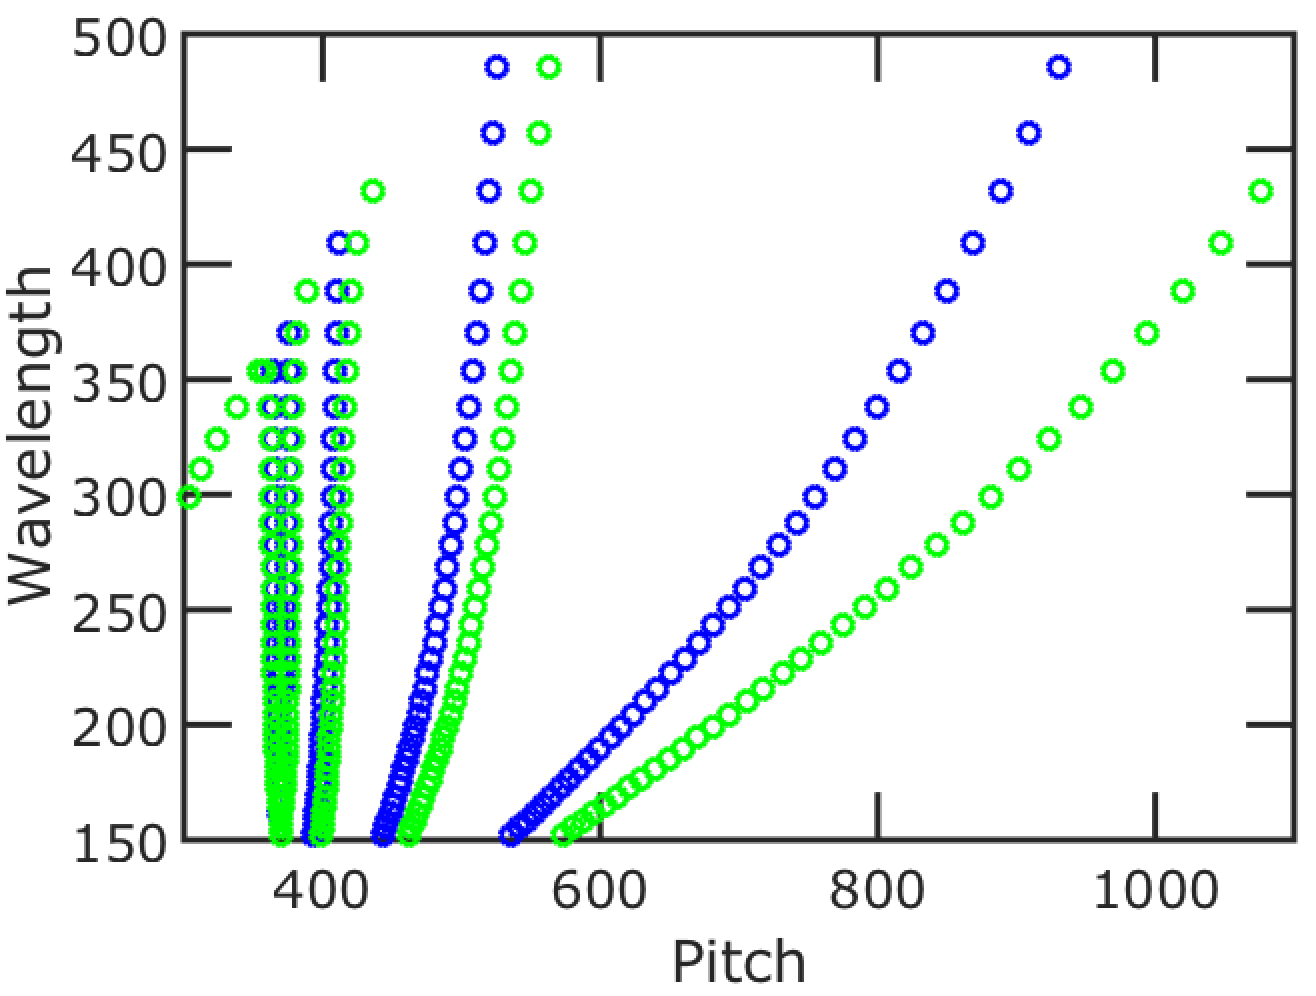
\includegraphics[scale=.4]{Figures/HemispherePaperWavelength2}
\caption{Guided Waveguide modes.}
\vspace{-10pt}
\end{figure}

\begin{figure}[H]
\centering 
\vspace{-10pt}
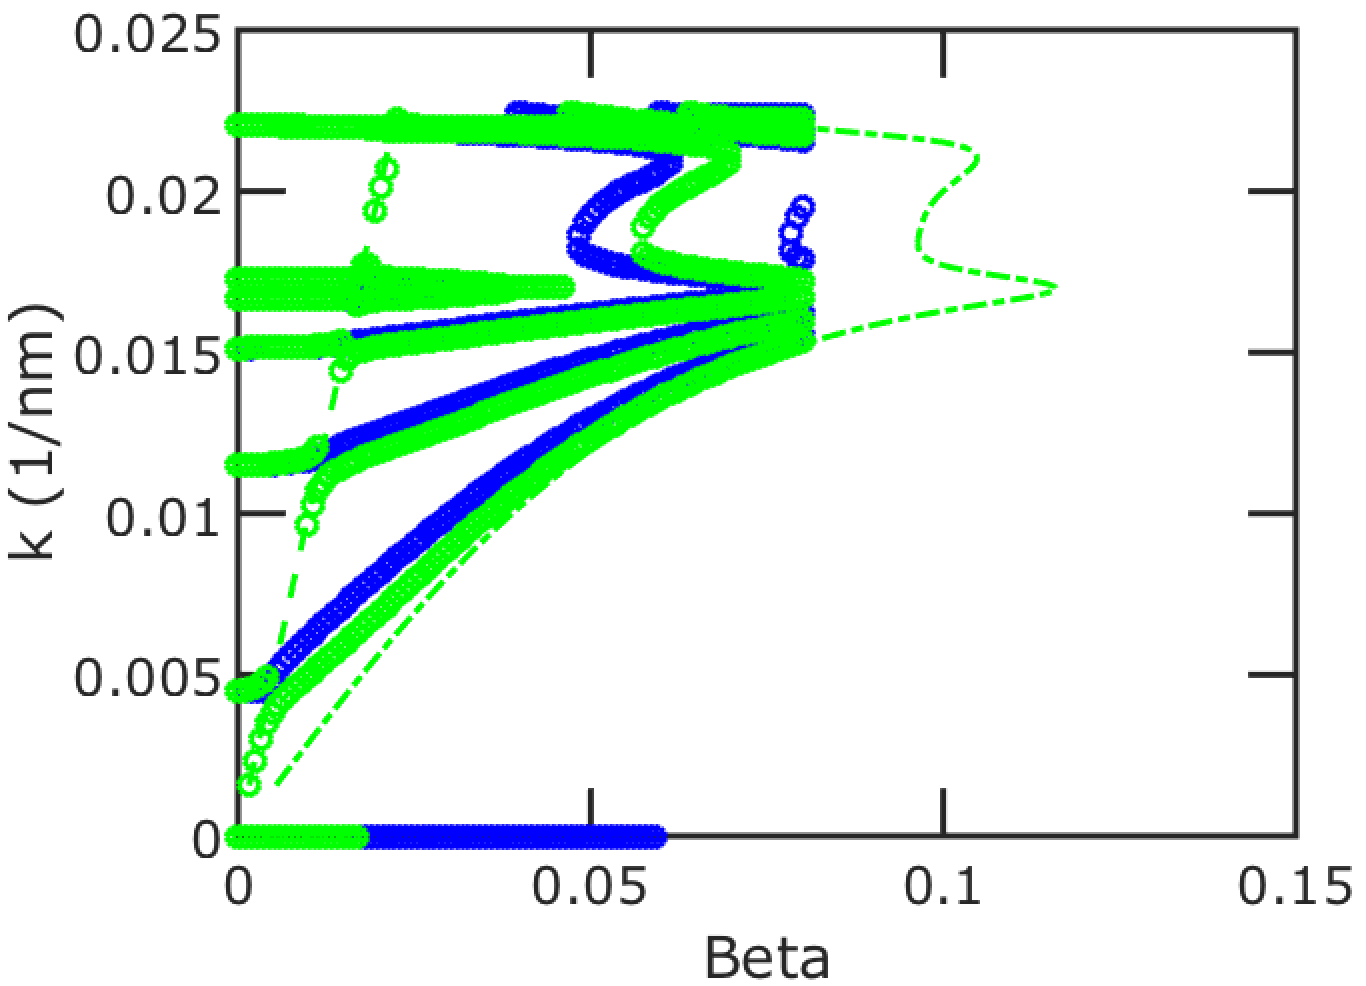
\includegraphics[scale=.4]{Figures/HemispherePaperKvsBeta}
\caption{}
\vspace{-10pt}
\end{figure}

\begin{figure}[H]
\centering 
\vspace{-10pt}
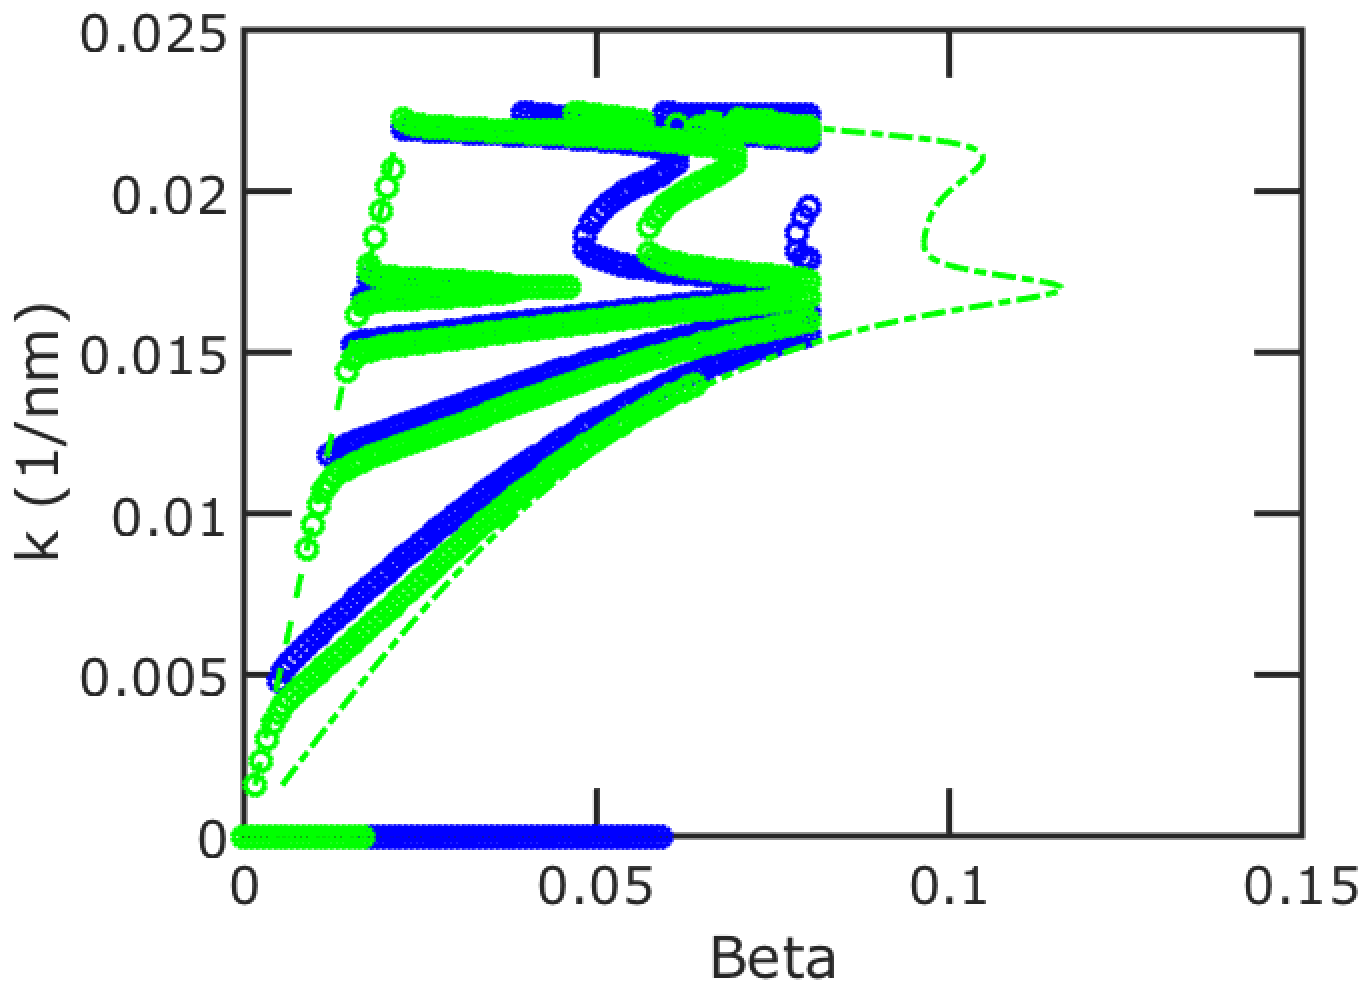
\includegraphics[scale=.4]{Figures/HemispherePaperKvsBetaYariv}
\caption{Using Yariv's equations}
\vspace{-10pt}
\end{figure}

%\subsection{Our Double Sided Metal Nanomesh Paper}



\subsection{Our Double Sided Metal Nanomesh Paper}

\begin{figure}[H]
\centering 
\vspace{-10pt}
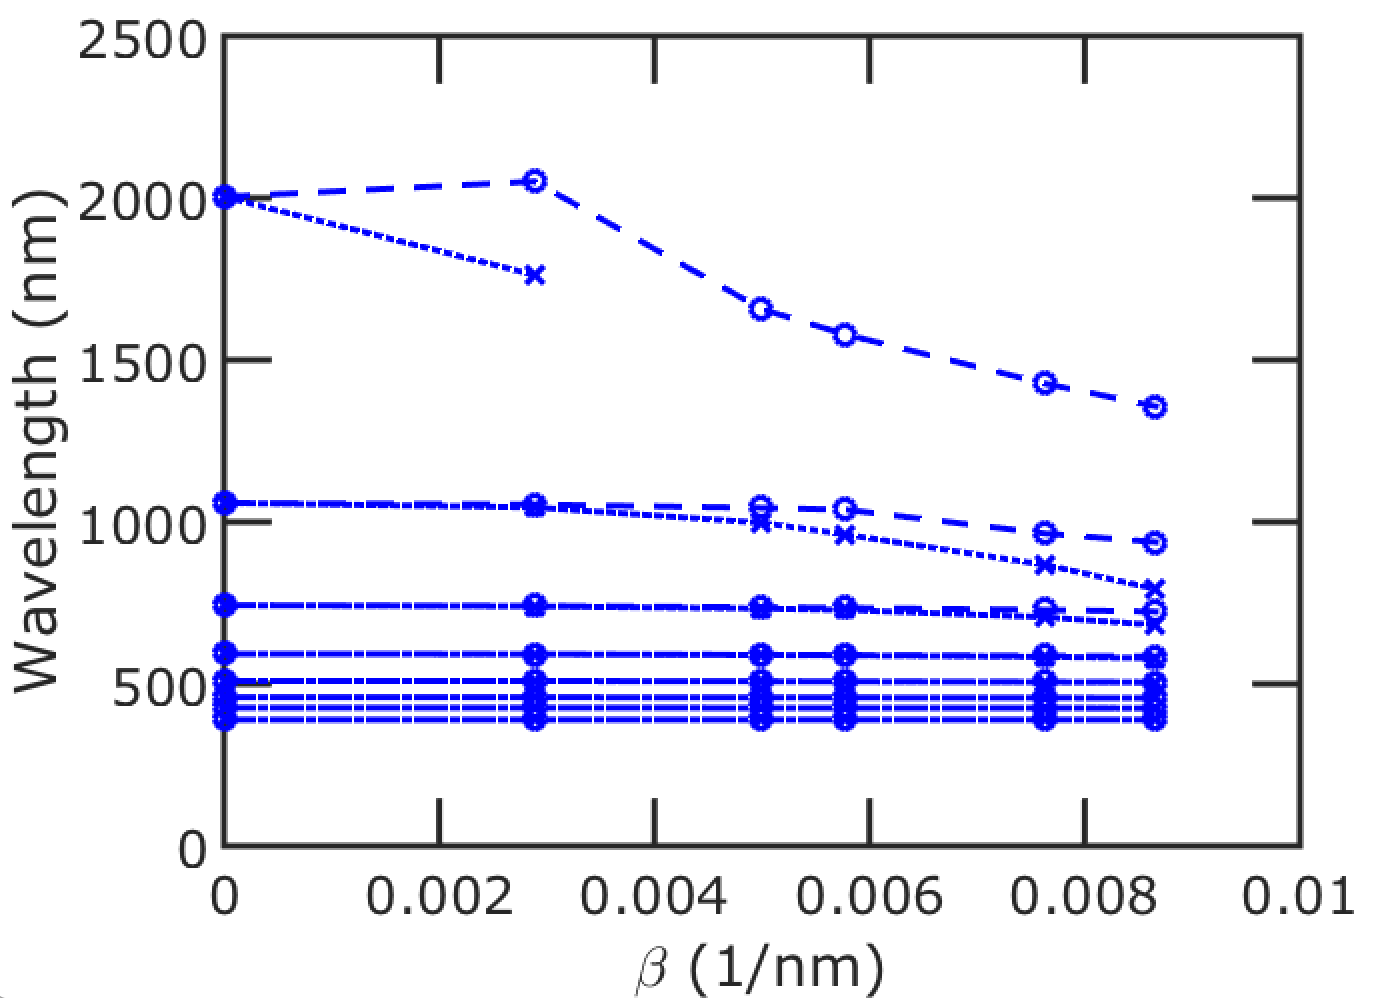
\includegraphics[scale=.4]{Figures/DoubleSidedMetalNanomeshPaper}
\vspace{-10pt}
\end{figure}

%\begin{figure}[H]
%\centering 
%\vspace{-10pt}
%\includegraphics[scale=.4]{Figures/DoubleSidedMetalNanomeshPaper2}
%\vspace{-10pt}
%\end{figure}


\section{Both sides metal}

\section{Yariv}

\subsection{Symmetric Slab Waveguides}
\subsubsection{Guided TE Modes}

\begin{equation}
h = \left [ \left ( \frac{n_2 \omega}{c} \right )^2 - \beta^2 \right ] ^{1/2}
\end{equation}

\begin{equation}
q = \left [ \beta^2 -  \left ( \frac{n_1 \omega}{c} \right )^2 \right ] ^{1/2}
\end{equation}

The symmetric modes are
\begin{equation}
h \tan (\frac{1}{2} h d ) = q
\end{equation}

The antisymmetric modes are
\begin{equation}
h \cot ( \frac{1}{2} h d ) = - q.
\end{equation}

The two equations can be combined
\begin{equation}
\tan (h d) = \frac{2 h q}{h^2 - q^2}
\end{equation}
For $\beta = 0$, the symmetric modes are 
\begin{equation}
 \tan (\frac{1}{2} n_2 k d) = i \frac{n_1}{n_2}
\end{equation}
or 
\begin{equation}
 \cot (\frac{1}{2} n_2 k d) = -i \frac{n_2}{n_1}
\end{equation}
and the antisymmetric modes are 
\begin{equation}
 \cot (\frac{1}{2} n_2 k d) = - i \frac{n_1}{n_2}
\end{equation}
or 
\begin{equation}
 \tan (\frac{1}{2} n_2 k d) = i \frac{n_2}{n_1}
\end{equation}
\blue{Note that these equations are slightly different from Linyou's.
Linyou's equations are for the even mode, 
$\cot (\frac{1}{2} n_2 k d ) = i \frac{n_2}{n_1} $
and the odd mode, 
$
\tan (\frac{1}{2} n_2 k d ) = - i \frac{n_2}{n_1} $.}

Compare this with the previous equations.  $k_{2x} = h$.  
However, $k_{1x} = i q$.  
When $\beta = 0$, $q = i n_1 k$ and $k_{x} = n_1 k$.  
The symmetric mode is 
\begin{equation}
k_{2x} \tan (\frac{1}{2} k_{2x} d ) = - i k_x.
\end{equation}
and the antisymmetric mode is
\begin{equation}
k_{2x} \cot (\frac{1}{2} k_{2x} d ) = i k_x
\end{equation}

For bound or guided modes, use $q$.  
For radiation modes, use $k_{1x}$.  


Using previous notation, 
\begin{equation}
k_{Si} = \left [ \left ( \frac{n_2 \omega}{c} \right )^2 - \beta^2 \right ] ^{1/2}
\end{equation}
\begin{equation}
k_{x} = \left [ \beta^2 -  \left ( \frac{n_1 \omega}{c} \right )^2 \right ] ^{1/2}
\end{equation}


\subsubsection{Guided TM Modes}

\blue{The even modes are really odd, since the magnetic field is a pseudovector.}
The even modes are 
\begin{equation}
h \tan (\frac{1}{2} h d ) = \frac{n_2^2}{n_1^2} q
\end{equation}
The odd modes are 
\begin{equation}
h \cot (\frac{1}{2} h d ) = \frac{n_2^2}{n_1^2} q
\end{equation}
The two equations can be combined
\begin{equation}
\tan (h d) = \frac{2 h \bar{q}}{h^2 - \bar{q}^2}
\end{equation}
where 
\begin{equation}
\bar{q} = \frac{n_2^2}{n_1^2} q
\end{equation}

\subsection{With Back Metal}

On metal, the modes are simply the odd modes with the $1/2$ removed
For TE modes, 
\begin{equation}
h \cot ( h  d) = -q
\end{equation}

For TM modes, 
\begin{equation}
h \tan ( h d ) = \frac{n_2^2}{n_1^2} q
\end{equation}

\subsection{Assymmetric Waveguides}

\begin{equation}
h = \left [ \left ( \frac{n_2 \omega}{c} \right )^2 - \beta^2 \right ] ^{1/2}
\end{equation}

\begin{equation}
q = \left [ \beta^2 -  \left ( \frac{n_1 \omega}{c} \right )^2 \right ] ^{1/2}
\end{equation}

\begin{equation}
p = \left [ \left ( \frac{n_3 \omega}{c} \right )^2 - \beta^2 \right ] ^{1/2}
\end{equation}

The TE modes are given by 
\begin{align}
\tan (h t) &=  \frac{p + q}{h ( 1 - pq/h^2)} \\
\tan (h t) &=  \frac{h (p + q)}{h^2 - pq}
\end{align}
This is the same formula given in 
 \cite{Tikhodeev:02}
 where $\bar{\beta} = h$, $\beta_s = p$, and $\beta = q$.
 
For TM modes, 
\begin{align}
\tan (h t) &=  \frac{h (\bar{p} + \bar{q})}{(h^2 - \bar{p} \bar{q})} \\
\end{align}
$\bar{p} = \frac{n_2^2}{n_3^2} p$
and $\bar{q} = \frac{n_2^2}{n_1^2} q$


Rearranging, we get
\begin{align}
\tan (h t) &=  \frac{\bar{\epsilon} h (p + \epsilon_s q)}{\epsilon_s h^2 - \bar{\epsilon}^2 \bar{q}} \\
\end{align}
which is the same as in  \cite{Tikhodeev:02}.




%\blue{Some issues with some modes missing.}

\bibliographystyle{IEEEtran}
\bibliography{../../../help/BibFiles/Photodetector,../../../help/BibFiles/SiliconPV,../../../help/BibFiles/Nanosphere,../../../help/BibFiles/Plasmonics,../../../help/BibFiles/PDOS}


\end{document}
